% This LaTeX document needs to be compiled with XeLaTeX.
\documentclass[
  10
]{article}
\usepackage[margin=2cm,includehead=true,includefoot=true,centering,]{geometry}
\usepackage{xcolor}
\usepackage{ucharclasses}
\usepackage{hyperref}
\usepackage{amsmath,amssymb}
\usepackage{amsfonts}
\usepackage[version=4]{mhchem}
\usepackage{stmaryrd}
\usepackage{bbold}
\usepackage{polyglossia}
\usepackage{fontspec}
\usepackage[fontset=none]{ctex}
\usepackage[export]{adjustbox}
\usepackage{tabularx}
\usepackage{booktabs}

\usepackage{setspace}
\setstretch{1.2}
\setcounter{secnumdepth}{3}
\setcounter{tocdepth}{3}

\makeatletter
\@ifundefined{KOMAClassName}{% if non-KOMA class
  \IfFileExists{parskip.sty}{%
    \usepackage{parskip}
  }{% else
    \setlength{\parindent}{0pt}
    \setlength{\parskip}{6pt plus 2pt minus 1pt}}
}{% if KOMA class
  \KOMAoptions{parskip=half}}
\makeatother
\usepackage{color}
\usepackage{fancyvrb}
\newcommand{\VerbBar}{|}
\newcommand{\VERB}{\Verb[commandchars=\\\{\}]}
\DefineVerbatimEnvironment{Highlighting}{Verbatim}{commandchars=\\\{\}}
% Add ',fontsize=\small' for more characters per line
\newenvironment{Shaded}{}{}
\newcommand{\AlertTok}[1]{\textcolor[rgb]{1.00,0.00,0.00}{\textbf{#1}}}
\newcommand{\AnnotationTok}[1]{\textcolor[rgb]{0.38,0.63,0.69}{\textbf{\textit{#1}}}}
\newcommand{\AttributeTok}[1]{\textcolor[rgb]{0.49,0.56,0.16}{#1}}
\newcommand{\BaseNTok}[1]{\textcolor[rgb]{0.25,0.63,0.44}{#1}}
\newcommand{\BuiltInTok}[1]{\textcolor[rgb]{0.00,0.50,0.00}{#1}}
\newcommand{\CharTok}[1]{\textcolor[rgb]{0.25,0.44,0.63}{#1}}
\newcommand{\CommentTok}[1]{\textcolor[rgb]{0.38,0.63,0.69}{\textit{#1}}}
\newcommand{\CommentVarTok}[1]{\textcolor[rgb]{0.38,0.63,0.69}{\textbf{\textit{#1}}}}
\newcommand{\ConstantTok}[1]{\textcolor[rgb]{0.53,0.00,0.00}{#1}}
\newcommand{\ControlFlowTok}[1]{\textcolor[rgb]{0.00,0.44,0.13}{\textbf{#1}}}
\newcommand{\DataTypeTok}[1]{\textcolor[rgb]{0.56,0.13,0.00}{#1}}
\newcommand{\DecValTok}[1]{\textcolor[rgb]{0.25,0.63,0.44}{#1}}
\newcommand{\DocumentationTok}[1]{\textcolor[rgb]{0.73,0.13,0.13}{\textit{#1}}}
\newcommand{\ErrorTok}[1]{\textcolor[rgb]{1.00,0.00,0.00}{\textbf{#1}}}
\newcommand{\ExtensionTok}[1]{#1}
\newcommand{\FloatTok}[1]{\textcolor[rgb]{0.25,0.63,0.44}{#1}}
\newcommand{\FunctionTok}[1]{\textcolor[rgb]{0.02,0.16,0.49}{#1}}
\newcommand{\ImportTok}[1]{\textcolor[rgb]{0.00,0.50,0.00}{\textbf{#1}}}
\newcommand{\InformationTok}[1]{\textcolor[rgb]{0.38,0.63,0.69}{\textbf{\textit{#1}}}}
\newcommand{\KeywordTok}[1]{\textcolor[rgb]{0.00,0.44,0.13}{\textbf{#1}}}
\newcommand{\NormalTok}[1]{#1}
\newcommand{\OperatorTok}[1]{\textcolor[rgb]{0.40,0.40,0.40}{#1}}
\newcommand{\OtherTok}[1]{\textcolor[rgb]{0.00,0.44,0.13}{#1}}
\newcommand{\PreprocessorTok}[1]{\textcolor[rgb]{0.74,0.48,0.00}{#1}}
\newcommand{\RegionMarkerTok}[1]{#1}
\newcommand{\SpecialCharTok}[1]{\textcolor[rgb]{0.25,0.44,0.63}{#1}}
\newcommand{\SpecialStringTok}[1]{\textcolor[rgb]{0.73,0.40,0.53}{#1}}
\newcommand{\StringTok}[1]{\textcolor[rgb]{0.25,0.44,0.63}{#1}}
\newcommand{\VariableTok}[1]{\textcolor[rgb]{0.10,0.09,0.49}{#1}}
\newcommand{\VerbatimStringTok}[1]{\textcolor[rgb]{0.25,0.44,0.63}{#1}}
\newcommand{\WarningTok}[1]{\textcolor[rgb]{0.38,0.63,0.69}{\textbf{\textit{#1}}}}
\usepackage{longtable,booktabs,array}
\newcounter{none} % for unnumbered tables
\usepackage{multirow}
\usepackage{calc} % for calculating minipage widths
% Correct order of tables after \paragraph or \subparagraph
\usepackage{etoolbox}
\makeatletter
\patchcmd\longtable{\par}{\if@noskipsec\mbox{}\fi\par}{}{}
\makeatother
% Allow footnotes in longtable head/foot
\IfFileExists{footnotehyper.sty}{\usepackage{footnotehyper}}{\usepackage{footnote}}
\makesavenoteenv{longtable}
\usepackage{graphicx}
\makeatletter
\newsavebox\pandoc@box
\newcommand*\pandocbounded[1]{% scales image to fit in text height/width
  \sbox\pandoc@box{#1}%
  \Gscale@div\@tempa{\textheight}{\dimexpr\ht\pandoc@box+\dp\pandoc@box\relax}%
  \Gscale@div\@tempb{\linewidth}{\wd\pandoc@box}%
  \ifdim\@tempb\p@<\@tempa\p@\let\@tempa\@tempb\fi% select the smaller of both
  \ifdim\@tempa\p@<\p@\scalebox{\@tempa}{\usebox\pandoc@box}%
  \else\usebox{\pandoc@box}%
  \fi%
}
% Set default figure placement to htbp
\def\fps@figure{htbp}
\makeatother
\setlength{\emergencystretch}{3em} % prevent overfull lines
\providecommand{\tightlist}{%
  \setlength{\itemsep}{0pt}\setlength{\parskip}{0pt}}


\hypersetup{colorlinks=true, linkcolor=blue, filecolor=magenta, urlcolor=cyan,}
\urlstyle{same}

\usepackage{colortbl}
\definecolor{table-row-color}{HTML}{999999}
\definecolor{table-rule-color}{HTML}{999999}
%\arrayrulecolor{black!40}
\arrayrulecolor{table-rule-color}     % color of \toprule, \midrule, \bottomrule
\setlength{\aboverulesep}{0pt}
\setlength{\belowrulesep}{0pt}


\setotherlanguages{english}
\IfFontExistsTF{Source Han Serif CN}
{\setCJKmainfont{Source Han Serif CN}\setCJKmonofont{Source Han Serif CN}\newfontfamily\chinesefont{Source Han Serif CN}}
{\IfFontExistsTF{Noto Serif CJK SC}
  {\setCJKmainfont{Noto Serif CJK SC}\setCJKmonofont{Noto Serif CJK SC}\newfontfamily\chinesefont{Noto Serif CJK SC}}
  {\IfFontExistsTF{PingFang SC}
    {\setCJKmainfont{PingFang SC}\setCJKmonofont{PingFang SC}\newfontfamily\chinesefont{PingFang SC}}
    {\IfFontExistsTF{SimSun}
      {\setCJKmainfont{SimSun}\setCJKmonofont{SimSun}\newfontfamily\chinesefont{SimSun}}
    {\IfFontExistsTF{FangSong}
      {\setCJKmainfont{FangSong}\setCJKmonofont{FangSong}\newfontfamily\chinesefont{FangSong}}
      {\setCJKmainfont{Arial Unicode MS}\setCJKmonofont{Arial Unicode MS}\newfontfamily\chinesefont{Arial Unicode MS}}
}}}}
\IfFontExistsTF{Times New Roman}
{\setmainfont{Times New Roman}\newfontfamily\englishfont{Times New Roman}}
{\IfFontExistsTF{Liberation Serif}
  {\setmainfont{Liberation Serif}\newfontfamily\englishfont{Liberation Serif}}
  {\IfFontExistsTF{DejaVu Serif}
    {\setmainfont{DejaVu Serif}\newfontfamily\englishfont{DejaVu Serif}}
    {\setmainfont{Arial}\newfontfamily\englishfont{Arial}}
}}


\author{}
\date{}

\begin{document}


\begin{center}
{\LARGE DeepSeek-V4：\par}
\vspace{0.4em}
{\Large 迈向高效的百万 Token 上下文智能\par}
\vspace{0.8em}
DeepSeek-AI research@deepseek.com
\end{center}

\section*{摘要}
\addcontentsline{toc}{section}{摘要}

我们发布了 DeepSeek-V4 系列的预览版本，其中包括两款强大的混合专家（MoE）语言模型：拥有 1.6T 参数（49B 激活）的 DeepSeek-V4-Pro，以及拥有 284B 参数（13B 激活）的 DeepSeek-V4-Flash；二者都支持一百万 Token 的上下文长度。DeepSeek-V4 系列在架构与优化方面包含若干关键升级：（1）将压缩稀疏注意力（CSA）与重度压缩注意力（HCA）结合的混合注意力架构，以提升长上下文效率；（2）增强传统残差连接的流形约束超连接（mHC）；（3）用于更快收敛和更高训练稳定性的 Muon 优化器。我们在超过 32T 的多样化高质量 Token 上对两个模型进行了预训练，随后采用全面的后训练流水线来释放并进一步增强其能力。DeepSeek-V4-Pro-Max 作为 DeepSeek-V4-Pro 的最高推理力度模式，重新定义了开源模型的最新水平，在核心任务上超越了其前代。同时，DeepSeek-V4 系列在长上下文场景下也极为高效。在一百万 Token 的上下文设定中，相比 DeepSeek-V3.2，DeepSeek-V4-Pro 的单 Token 推理 FLOPs 仅为其 \(27\%\)，KV 缓存仅为其 \(10\%\)。这使我们能够常态化支持一百万 Token 上下文，从而让长时程任务和进一步的测试时扩展更加可行。模型检查点可在 \url{https://huggingface.co/collections/deepseek-ai/deepseek-v4} 获取。

\pandocbounded{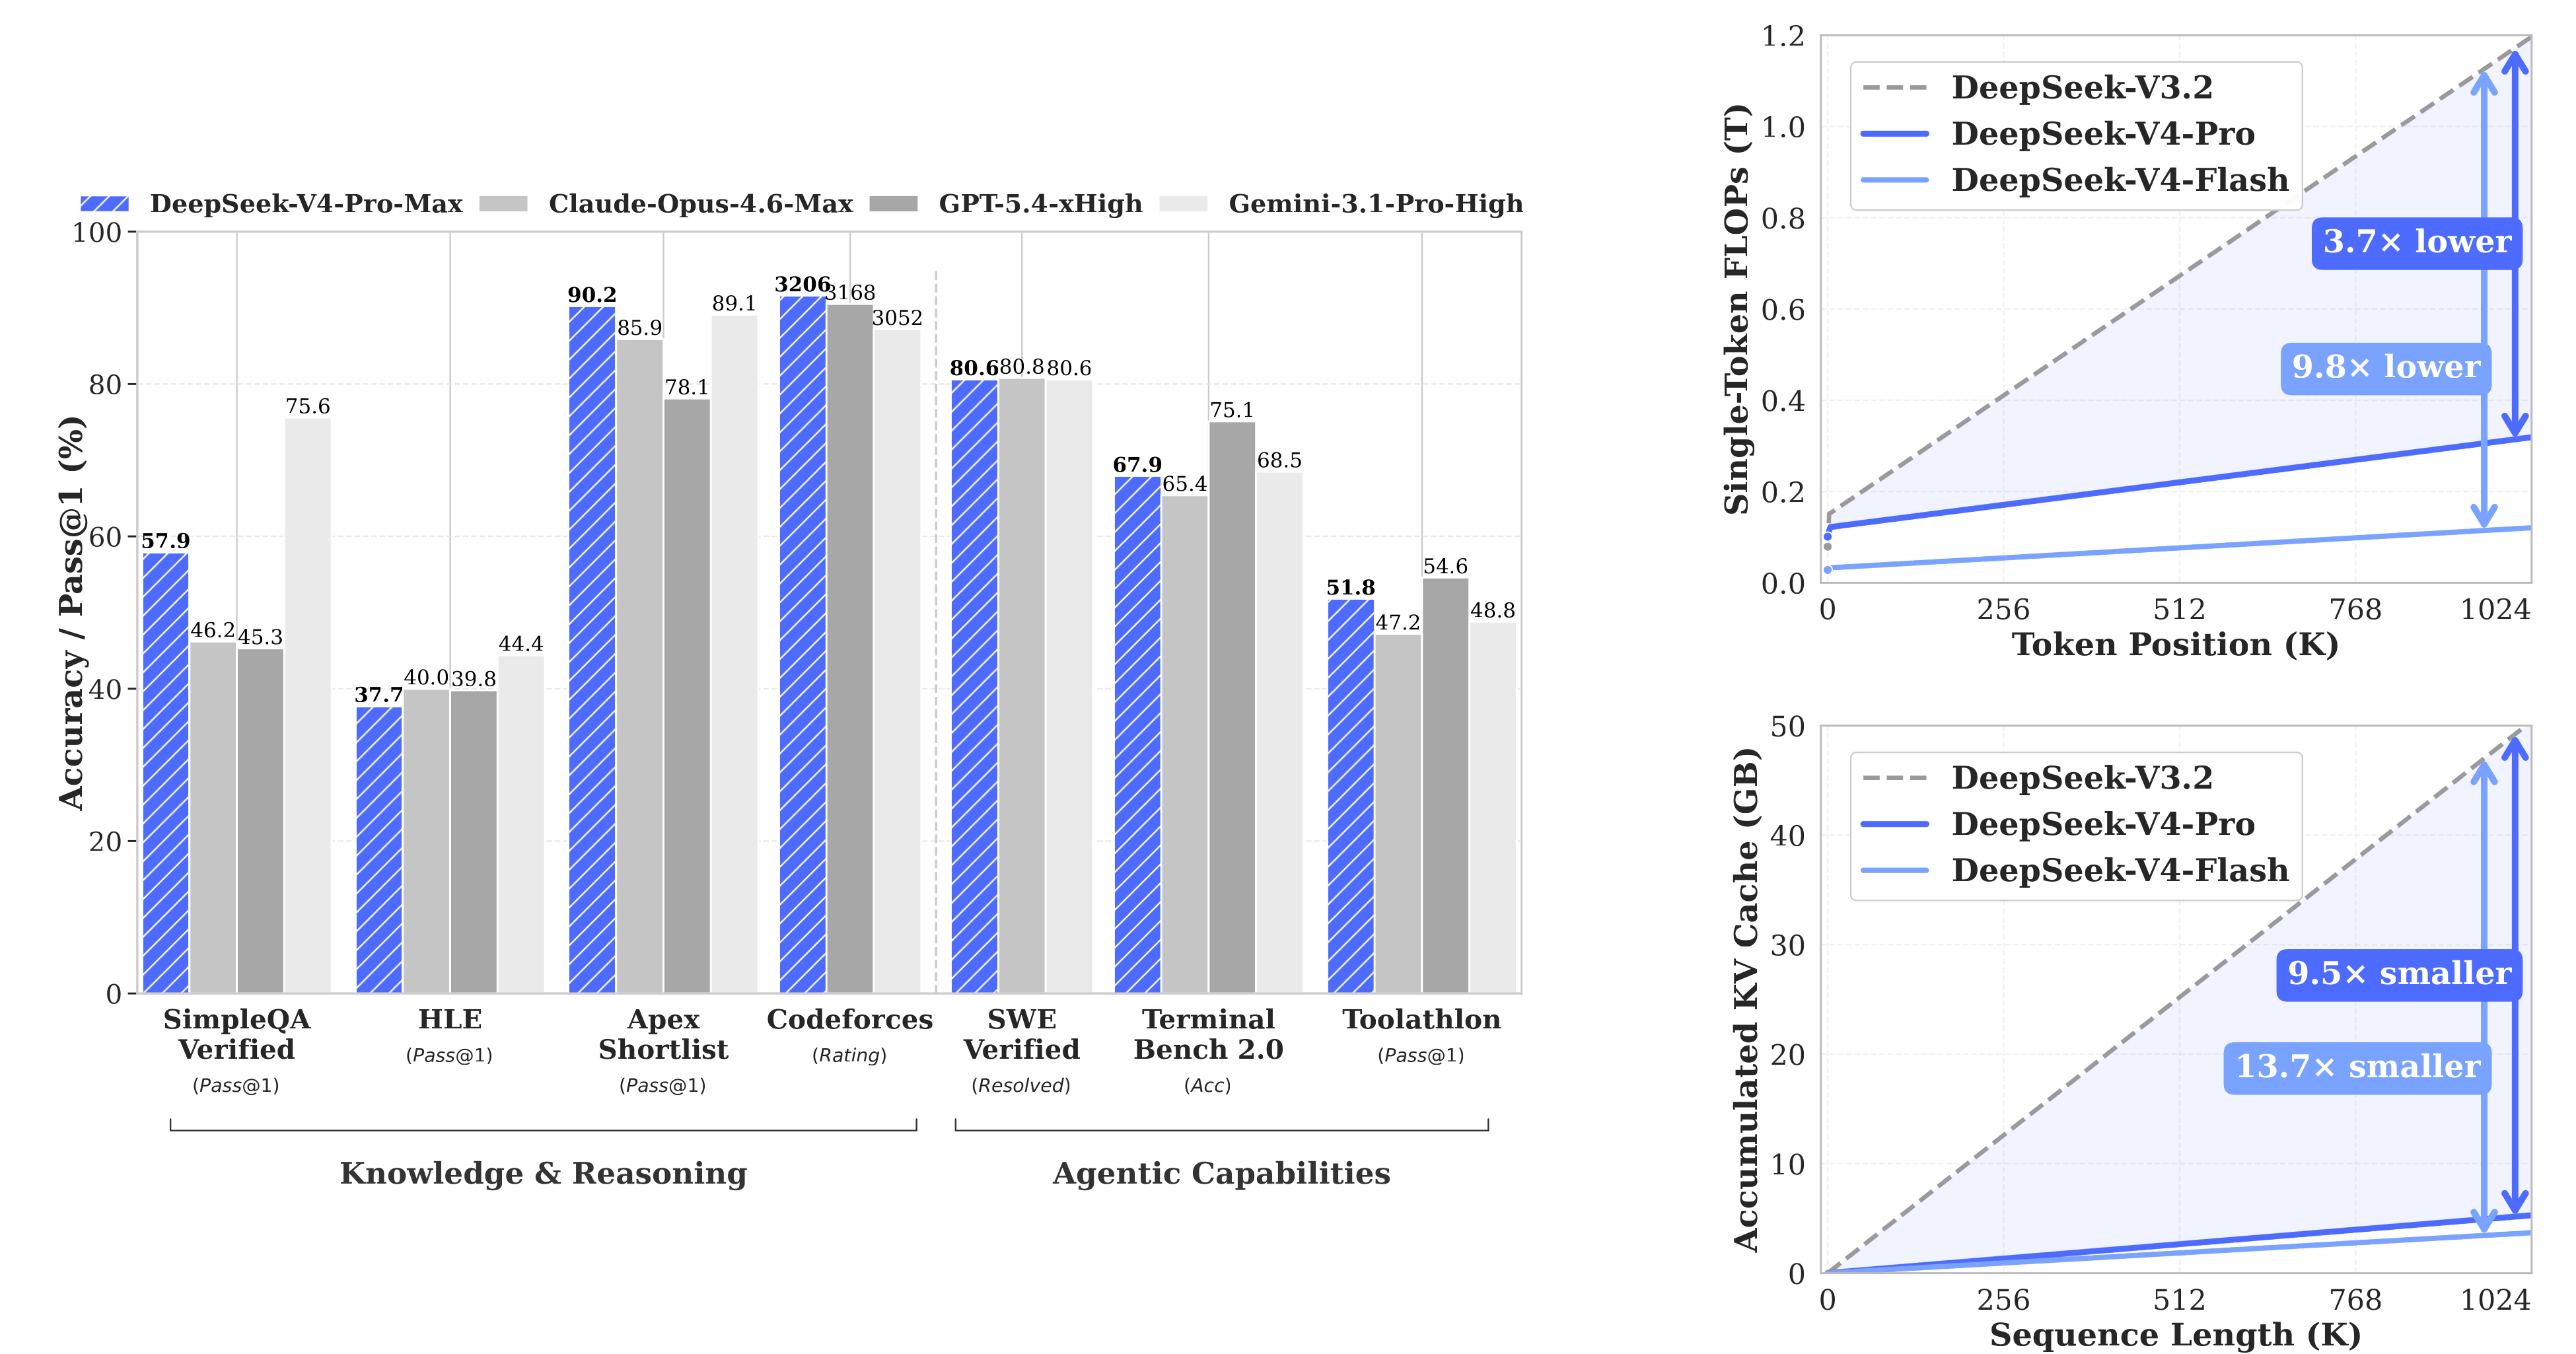
\includegraphics[keepaspectratio,alt={image}]{images_hi/Figure1_hi.png}}

图 1 \textbar{} 左：DeepSeek-V4-Pro-Max 与其对比模型的基准性能。右：DeepSeek-V4 系列与 DeepSeek-V3.2 的推理 FLOPs 与 KV 缓存大小。

\tableofcontents
\clearpage

\input{parts/part1_cn.md}
\input{parts/part2_cn.md}
\input{parts/part3_cn.md}
\input{parts/part4_cn.md}
\input{parts/conclusion_cn.md}

\phantomsection
\section*{References}\label{references}

AA. Gdpval-aa leaderboard, 2025. URL
https://artificialanalysis.ai/methodology/intelligence-benchmarking\#gdpval-aa.

T. Achim, A. Best, A. Bietti, K. Der, M. Fédérico, S. Gukov, D.
Halpern-Leistner, K. Henningsgard,Y. Kudryashov, A. Meiburg, et
al.~Aristotle: Imo-level automated theorem proving. arXivpreprint
arXiv:2510.01346, 2025.

A. Agache, M. Brooker, A. Florescu, A. Iordache, A. Liguori, R.
Neugebauer, P. Piwonka, andD.-M. Popa. Firecracker: lightweight
virtualization for serverless applications. In Proceedingsof the 17th
Usenix Conference on Networked Systems Design and Implementation,
NSDI'20,page 419--434, USA, 2020. USENIX Association. ISBN
9781939133137.

O. J. Aimuyo, B. Oh, and R. Singh. Flashmoe: Fast distributed moe in a
single kernel. Advancesin Neural Information Processing Systems, 2025.
URL https://neurips.cc/virtual/2025/poster/119124.

J. Ainslie, J. Lee-Thorp, M. de Jong, Y. Zemlyanskiy, F. Lebrón, and S.
Sanghai. Gqa: Traininggeneralized multi-query transformer models from
multi-head checkpoints. arXiv preprintarXiv:2305.13245, 2023.

J. Asher. LeanExplore: A search engine for Lean 4 declarations, 2025.
URL https://arxiv.org/abs/2506.11085.

Y. Bai, Y. Bao, G. Chen, J. Chen, N. Chen, R. Chen, Y. Chen, Y. Chen, Y.
Chen, Z. Chen, J. Cui,H. Ding, M. Dong, A. Du, C. Du, D. Du, Y. Du, Y.
Fan, Y. Feng, K. Fu, B. Gao, H. Gao, P. Gao,T. Gao, X. Gu, L. Guan, H.
Guo, J. Guo, H. Hu, X. Hao, T. He, W. He, W. He, C. Hong, Y. Hu,Z. Hu,
W. Huang, Z. Huang, Z. Huang, T. Jiang, Z. Jiang, X. Jin, Y. Kang, G.
Lai, C. Li, F. Li,H. Li, M. Li, W. Li, Y. Li, Y. Li, Z. Li, Z. Li, H.
Lin, X. Lin, Z. Lin, C. Liu, C. Liu, H. Liu, J. Liu,J. Liu, L. Liu, S.
Liu, T. Y. Liu, T. Liu, W. Liu, Y. Liu, Y. Liu, Y. Liu, Y. Liu, Z. Liu,
E. Lu, L. Lu,S. Ma, X. Ma, Y. Ma, S. Mao, J. Mei, X. Men, Y. Miao, S.
Pan, Y. Peng, R. Qin, B. Qu, Z. Shang,L. Shi, S. Shi, F. Song, J. Su, Z.
Su, X. Sun, F. Sung, H. Tang, J. Tao, Q. Teng, C. Wang, D. Wang,F. Wang,
and H. Wang. Kimi K2: open agentic intelligence. CoRR, abs/2507.20534,
2025a.URL https://doi.org/10.48550/arXiv.2507.20534.

Y. Bai, S. Tu, J. Zhang, H. Peng, X. Wang, X. Lv, S. Cao, J. Xu, L. Hou,
Y. Dong, et al.~Longbenchv2: Towards deeper understanding and reasoning
on realistic long-context multitasks. InProceedings of the 63rd Annual
Meeting of the Association for Computational Linguistics(Volume 1: Long
Papers), pages 3639--3664, 2025b.

M. Balunovi´c, J. Dekoninck, I. Petrov, N. Jovanovi´c, and M. Vechev.
Matharena: Evaluating llmson uncontaminated math competitions.
Proceedings of the Neural Information ProcessingSystems Track on
Datasets and Benchmark, 2025.

C. Bandi, B. Hertzberg, G. Boo, T. Polakam, J. Da, S. Hassaan, M.
Sharma, A. Park, E. Hernandez,D. Rambado, et al.~Mcp-atlas: A
large-scale benchmark for tool-use competency with realmcp servers.
arXiv preprint arXiv:2602.00933, 2026.

F. Bellard. Qemu, a fast and portable dynamic translator. In Proceedings
of the AnnualConference on USENIX Annual Technical Conference, ATEC '05,
page 41, USA, 2005. USENIXAssociation.

I. Bello, H. Pham, Q. V. Le, M. Norouzi, and S. Bengio. Neural
combinatorial optimization withreinforcement learning, 2017. URL
https://openreview.net/forum?id=rJY3vK9eg.

J. Chen, W. Chen, J. Du, J. Hu, Z. Jiang, A. Jie, X. Jin, X. Jin, C. Li,
W. Shi, Z. Wang, M. Wang,C. Wei, S. Wei, H. Xin, F. Yang, W. Gao, Z.
Yuan, T. Zhan, Z. Zheng, T. Zhou, and T. H.Zhu. Seed-prover 1.5:
Mastering undergraduate-level theorem proving via learning
fromexperience, 2025. URL https://arxiv.org/abs/2512.17260.

M. Chen, J. Tworek, H. Jun, Q. Yuan, H. P. de Oliveira Pinto, J. Kaplan,
H. Edwards, Y. Burda,N. Joseph, G. Brockman, A. Ray, R. Puri, G.
Krueger, M. Petrov, H. Khlaaf, G. Sastry, P. Mishkin,B. Chan, S. Gray,
N. Ryder, M. Pavlov, A. Power, L. Kaiser, M. Bavarian, C. Winter, P.
Tillet,F. P. Such, D. Cummings, M. Plappert, F. Chantzis, E. Barnes, A.
Herbert-Voss, W. H. Guss,A. Nichol, A. Paino, N. Tezak, J. Tang, I.
Babuschkin, S. Balaji, S. Jain, W. Saunders, C. Hesse,A. N. Carr, J.
Leike, J. Achiam, V. Misra, E. Morikawa, A. Radford, M. Knight, M.
Brundage,M. Murati, K. Mayer, P. Welinder, B. McGrew, D. Amodei, S.
McCandlish, I. Sutskever, andW. Zaremba. Evaluating large language
models trained on code. CoRR, abs/2107.03374, 2021.URL
https://arxiv.org/abs/2107.03374.

T. Chen, T. Moreau, Z. Jiang, L. Zheng, E. Yan, H. Shen, M. Cowan, L.
Wang, Y. Hu, L. Ceze,C. Guestrin, and A. Krishnamurthy. TVM: An
automated End-to-End optimizing com-piler for deep learning. In 13th
USENIX Symposium on Operating Systems Design andImplementation (OSDI
18), pages 578--594, Carlsbad, CA, Oct.~2018. USENIX Association.ISBN
978-1-939133-08-3. URL
https://www.usenix.org/conference/osdi18/presentation/chen.

A. Cheng, A. Jacovi, A. Globerson, B. Golan, C. Kwong, C. Alberti, C.
Tao, E. Ben-David, G. S.Tomar, L. Haas, et al.~The facts leaderboard: A
comprehensive benchmark for large languagemodel factuality. arXiv
preprint arXiv:2512.10791, 2025.

X. Cheng, W. Zeng, D. Dai, Q. Chen, B. Wang, Z. Xie, K. Huang, X. Yu, Z.
Hao, Y. Li, H. Zhang,H. Zhang, D. Zhao, and W. Liang. Conditional memory
via scalable lookup: A new axis ofsparsity for large language models.
CoRR, abs/2601.07372, 2026. doi: 10.48550/ARXIV.2601.07372. URL
https://doi.org/10.48550/arXiv.2601.07372.

K. Cobbe, V. Kosaraju, M. Bavarian, M. Chen, H. Jun, L. Kaiser, M.
Plappert, J. Tworek,J. Hilton, R. Nakano, et al.~Training verifiers to
solve math word problems. arXiv preprintarXiv:2110.14168, 2021.

D. Dai, C. Deng, C. Zhao, R. X. Xu, H. Gao, D. Chen, J. Li, W. Zeng, X.
Yu, Y. Wu, Z. Xie, Y. K.Li, P. Huang, F. Luo, C. Ruan, Z. Sui, and W.
Liang. Deepseekmoe: Towards ultimate expertspecialization in
mixture-of-experts language models. CoRR, abs/2401.06066, 2024.
URLhttps://doi.org/10.48550/arXiv.2401.06066.

T. Dao, D. Haziza, F. Massa, and G. Sizov. Flash-decoding for
long-context inference, 2023.
URLhttps://pytorch.org/blog/flash-decoding/.

L. De Moura and N. Bjørner. Z3: an efficient smt solver. In Proceedings
of the Theoryand Practice of Software, 14th International Conference on
Tools and Algorithms for theConstruction and Analysis of Systems,
TACAS'08/ETAPS'08, page 337--340, Berlin, Heidel-berg, 2008.
Springer-Verlag. ISBN 3540787992.

DeepSeek-AI. Deepseek-coder-v2: Breaking the barrier of closed-source
models in code intelli-gence. CoRR, abs/2406.11931, 2024. URL
https://doi.org/10.48550/arXiv.2406.11931.

DeepSeek-AI. Deepseek-v3 technical report. CoRR, abs/2412.19437, 2024.
URL https://doi.org/10.48550/arXiv.2412.19437.

DeepSeek-AI. Deepseek-v2: A strong, economical, and efficient
mixture-of-experts languagemodel. CoRR, abs/2405.04434, 2024. URL
https://doi.org/10.48550/arXiv.2405.04434.

DeepSeek-AI. Fire-flyer file system, 2025. URL
https://github.com/deepseek-ai/3FS.

DeepSeek-AI. Deepseek-r1 incentivizes reasoning in llms through
reinforcement learning. Nat.,645(8081):633--638, 2025. URL
https://doi.org/10.1038/s41586-025-09422-z.

DeepSeek-AI. Deepseek-v3.2: Pushing the frontier of open large language
models, 2025. URLhttps://arxiv.org/abs/2512.02556.

X. Deng, J. Da, E. Pan, Y. Y. He, C. Ide, K. Garg, N. Lauffer, A. Park,
N. Pasari, C. Rane, K. Sampath,M. Krishnan, S. Kundurthy, S. Hendryx, Z.
Wang, V. Bharadwaj, J. Holm, R. Aluri, C. B. C.Zhang, N. Jacobson, B.
Liu, and B. Kenstler. Swe-bench pro: Can ai agents solve
long-horizonsoftware engineering tasks?, 2025. URL
https://arxiv.org/abs/2509.16941.

H. Ding, Z. Wang, G. Paolini, V. Kumar, A. Deoras, D. Roth, and S.
Soatto. Fewer truncationsimprove language modeling. arXiv preprint
arXiv:2404.10830, 2024.

X. Dong, Y. Fu, S. Diao, W. Byeon, Z. CHEN, A. S. Mahabaleshwarkar,
S.-Y. Liu, M. V. keirsbilck,M.-H. Chen, Y. Suhara, Y. C. Lin, J. Kautz,
and P. Molchanov. Hymba: A hybrid-head archi-tecture for small language
models. In The Thirteenth International Conference on
LearningRepresentations, 2025. URL
https://openreview.net/forum?id=A1ztozypga.

X. Du, Y. Yao, K. Ma, B. Wang, T. Zheng, K. Zhu, M. Liu, Y. Liang, X.
Jin, Z. Wei, et al.~Supergpqa:Scaling llm evaluation across 285 graduate
disciplines. arXiv preprint arXiv:2502.14739, 2025.

D. Dua, Y. Wang, P. Dasigi, G. Stanovsky, S. Singh, and M. Gardner.
DROP: A reading compre-hension benchmark requiring discrete reasoning
over paragraphs. In J. Burstein, C. Doran, andT. Solorio, editors,
Proceedings of the 2019 Conference of the North American Chapter of
theAssociation for Computational Linguistics: Human Language
Technologies, NAACL-HLT2019, Minneapolis, MN, USA, June 2-7, 2019,
Volume 1 (Long and Short Papers), pages 2368--2378. Association for
Computational Linguistics, 2019. doi: 10.18653/V1/N19-1246.
URLhttps://doi.org/10.18653/v1/n19-1246.

X. Gao, M. Dong, X. Miao, W. Du, C. Yu, and H. Chen. Erofs: a
compression-friendly readonlyfile system for resource-scarce devices. In
Proceedings of the 2019 USENIX Conference onUsenix Annual Technical
Conference, USENIX ATC '19, page 149--162, USA, 2019. USENIXAssociation.
ISBN 9781939133038.

A. P. Gema, J. O. J. Leang, G. Hong, A. Devoto, A. C. M. Mancino, R.
Saxena, X. He, Y. Zhao,X. Du, M. R. G. Madani, C. Barale, R. McHardy, J.
Harris, J. Kaddour, E. van Krieken, andP. Minervini. Are we done with
mmlu? CoRR, abs/2406.04127, 2024. URL
https://doi.org/10.48550/arXiv.2406.04127.

F. Gloeckle, B. Y. Idrissi, B. Rozière, D. Lopez-Paz, and G. Synnaeve.
Better \& faster largelanguage models via multi-token prediction. In
Forty-first International Conference onMachine Learning, ICML 2024,
Vienna, Austria, July 21-27, 2024. OpenReview.net, 2024.
URLhttps://openreview.net/forum?id=pEWAcejiU2.

L. Haas, G. Yona, G. D'Antonio, S. Goldshtein, and D. Das. Simpleqa
verified: A reliablefactuality benchmark to measure parametric
knowledge. arXiv preprint arXiv:2509.07968,2025.

Y. He, S. Li, J. Liu, Y. Tan, W. Wang, H. Huang, X. Bu, H. Guo, C. Hu,
B. Zheng, et al.~Chi-nese simpleqa: A chinese factuality evaluation for
large language models. arXiv preprintarXiv:2411.07140, 2024.

D. Hendrycks, C. Burns, S. Basart, A. Zou, M. Mazeika, D. Song, and J.
Steinhardt. Measuringmassive multitask language understanding. arXiv
preprint arXiv:2009.03300, 2020.

D. Hendrycks, C. Burns, S. Kadavath, A. Arora, S. Basart, E. Tang, D.
Song, and J. Steinhardt. Mea-suring mathematical problem solving with
the math dataset. arXiv preprint arXiv:2103.03874,2021.

Y. Huang, Y. Bai, Z. Zhu, J. Zhang, J. Zhang, T. Su, J. Liu, C. Lv, Y.
Zhang, J. Lei, et al.~C-Eval: Amulti-level multi-discipline chinese
evaluation suite for foundation models. arXiv preprintarXiv:2305.08322,
2023.

D. Hupkes and N. Bogoychev. Multiloko: a multilingual local knowledge
benchmark for llmsspanning 31 languages. CoRR, abs/2504.10356, 2025.
doi: 10.48550/ARXIV.2504.10356.
URLhttps://doi.org/10.48550/arXiv.2504.10356.

B. Jacob, S. Kligys, B. Chen, M. Zhu, M. Tang, A. Howard, H. Adam, and
D. Kalenichenko.Quantization and training of neural networks for
efficient integer-arithmetic-only inference.In Proceedings of the IEEE
Conference on Computer Vision and Pattern Recognition (CVPR),June 2018.

N. Jain, K. Han, A. Gu, W.-D. Li, F. Yan, T. Zhang, S. Wang, A.
Solar-Lezama, K. Sen, and I. Stoica.Livecodebench: Holistic and
contamination free evaluation of large language models for code.arXiv
preprint arXiv:2403.07974, 2024.

K. Jordan, Y. Jin, V. Boza, J. You, F. Cesista, L. Newhouse, and J.
Bernstein. Muon: An optimizerfor hidden layers in neural networks. Cited
on, page 10, 2024.

M. Joshi, E. Choi, D. Weld, and L. Zettlemoyer. TriviaQA: A large scale
distantly supervised chal-lenge dataset for reading comprehension. In R.
Barzilay and M.-Y. Kan, editors, Proceedings ofthe 55th Annual Meeting
of the Association for Computational Linguistics (Volume 1: LongPapers),
pages 1601--1611, Vancouver, Canada, July 2017. Association for
ComputationalLinguistics. doi: 10.18653/v1/P17-1147. URL
https://aclanthology.org/P17-1147.

H. Li, Y. Yuan, R. Du, K. Ma, L. Liu, and W. Hsu. DADI: Block-Level
image service for agileand elastic application deployment. In 2020
USENIX Annual Technical Conference (USENIXATC 20), pages 727--740.
USENIX Association, July 2020. ISBN 978-1-939133-14-4.
URLhttps://www.usenix.org/conference/atc20/presentation/li-huiba.

H. Li, Y. Zhang, F. Koto, Y. Yang, H. Zhao, Y. Gong, N. Duan, and T.
Baldwin. CMMLU: Measur-ing massive multitask language understanding in
Chinese. arXiv preprint arXiv:2306.09212,2023.

J. Li, W. Zhao, J. Zhao, W. Zeng, H. Wu, X. Wang, R. Ge, Y. Cao, Y.
Huang, W. Liu, et al.~Thetool decathlon: Benchmarking language agents
for diverse, realistic, and long-horizon taskexecution. arXiv preprint
arXiv:2510.25726, 2025.

Y. Li, F. Wei, C. Zhang, and H. Zhang. EAGLE: speculative sampling
requires rethinkingfeature uncertainty. In Forty-first International
Conference on Machine Learning, ICML 2024,Vienna, Austria, July 21-27,
2024. OpenReview.net, 2024. URL
https://openreview.net/forum?id=1NdN7eXyb4.

J. Liu, J. Su, X. Yao, Z. Jiang, G. Lai, Y. Du, Y. Qin, W. Xu, E. Lu, J.
Yan, Y. Chen, H. Zheng,Y. Liu, S. Liu, B. Yin, W. He, H. Zhu, Y. Wang,
J. Wang, M. Dong, Z. Zhang, Y. Kang, H. Zhang,X. Xu, Y. Zhang, Y. Wu, X.
Zhou, and Z. Yang. Muon is scalable for LLM training.
CoRR,abs/2502.16982, 2025. URL
https://doi.org/10.48550/arXiv.2502.16982.

I. Loshchilov and F. Hutter. Decoupled weight decay regularization.
arXiv preprintarXiv:1711.05101, 2017.

K. Lu and T. M. Lab. On-policy distillation. Thinking Machines Lab:
Connectionism, 2025. doi:10.64434/tml.20251026.
https://thinkingmachines.ai/blog/on-policy-distillation.

Z. Lu, C. Li, Y. Shi, W. Shen, M. Yan, and F. Huang. Corpusqa: A 10
million token benchmarkfor corpus-level analysis and reasoning. arXiv
preprint arXiv:2601.14952, 2026.

T. Luong, D. Hwang, H. H. Nguyen, G. Ghiasi, Y. Chervonyi, I. Seo, J.
Kim, G. Bingham,J. Lee, S. Mishra, A. Zhai, C. H. Hu, H. Michalewski, J.
Kim, J. Ahn, J. Bae, X. Song, T. H.Trinh, Q. V. Le, and J. Jung. Towards
robust mathematical reasoning. In Proceedings ofthe 2025 Conference on
Empirical Methods in Natural Language Processing, 2025.
URLhttps://aclanthology.org/2025.emnlp-main.1794/.

M. A. Merrill, A. G. Shaw, N. Carlini, B. Li, H. Raj, I. Bercovich, L.
Shi, J. Y. Shin, T. Walshe, E. K.Buchanan, et al.~Terminal-bench:
Benchmarking agents on hard, realistic tasks in commandline interfaces.
arXiv preprint arXiv:2601.11868, 2026.

MiniMax. Meet minimax-m2, 2025. URL
https://github.com/MiniMax-AI/MiniMax-M2.

L. d.~Moura and S. Ullrich. The lean 4 theorem prover and programming
language. InInternational Conference on Automated Deduction, pages
625--635. Springer, 2021.

Y. Nesterov. A method of solving a convex programming problem with
convergence rate \(O ( 1 / k ^ { 2 } )\) .Soviet Mathematics Doklady,
27:372--376, 1983.

NVIDIA Corporation. cublas documentation, 2024. URL
https://docs.nvidia.com/cuda/cublas/. Version 12.4. Accessed:
2024-09-16.

OpenAI. Multilingual massive multitask language understanding (mmmlu),
2024a. URLhttps://huggingface.co/datasets/openai/MMMLU.

OpenAI. Openai mrcr: Long context multiple needle in a haystack
benchmark, 2024b. URLhttps://huggingface.co/datasets/openai/mrcr.

OpenAI. Learning to reason with llms, 2024c. URL
https://openai.com/index/learning-to-reason-with-llms.

OpenAI. Introducing SimpleQA, 2024d. URL
https://openai.com/index/introducing-simpleqa/.

OpenAI. Introducing SWE-bench verified we're releasing a human-validated
subset of swe-bench that more, 2024e. URL
https://openai.com/index/introducing-swe-bench-verified/.

OpenAI. gpt-oss-120b \& gpt-oss-20b model card. CoRR, abs/2508.10925,
2025. doi: 10.48550/ARXIV.2508.10925. URL
https://doi.org/10.48550/arXiv.2508.10925.

M. Osama, D. Merrill, C. Cecka, M. Garland, and J. D. Owens. Stream-k:
Work-centric paralleldecomposition for dense matrix-matrix
multiplication on the gpu. In Proceedings of the 28thACM SIGPLAN Annual
Symposium on Principles and Practice of Parallel Programming,pages
429--431, 2023.

T. Patwardhan, R. Dias, E. Proehl, G. Kim, M. Wang, O. Watkins, S. P.
Fishman, M. Aljubeh,P. Thacker, L. Fauconnet, et al.~Gdpval: Evaluating
ai model performance on real-worldeconomically valuable tasks. arXiv
preprint arXiv:2510.04374, 2025.

L. Phan, A. Gatti, Z. Han, N. Li, J. Hu, H. Zhang, C. B. C. Zhang, M.
Shaaban, J. Ling, S. Shi, et al.Humanity's last exam. arXiv preprint
arXiv:2501.14249, 2025.

W. Qi, Y. Yan, Y. Gong, D. Liu, N. Duan, J. Chen, R. Zhang, and M. Zhou.
Prophetnet: Predictingfuture n-gram for sequence-to-sequence
pre-training. In T. Cohn, Y. He, and Y. Liu, edi-tors, Findings of the
Association for Computational Linguistics: EMNLP 2020, Online
Event,16-20 November 2020, volume EMNLP 2020 of Findings of ACL, pages
2401--2410. Associa-tion for Computational Linguistics, 2020. URL
https://doi.org/10.18653/v1/2020.findings-emnlp.217.

Qwen. Qwen3 technical report. CoRR, abs/2505.09388, 2025. doi:
10.48550/ARXIV.2505.09388.URL https://doi.org/10.48550/arXiv.2505.09388.

S. Rajbhandari, J. Rasley, O. Ruwase, and Y. He. Zero: Memory
optimizations toward training tril-lion parameter models. In SC20:
International Conference for High Performance Computing,Networking,
Storage and Analysis, pages 1--16. IEEE, 2020.

J. K. Reed, Z. DeVito, H. He, A. Ussery, and J. Ansel. Torch.fx:
Practical program capture andtransformation for deep learning in python,
2022. URL https://arxiv.org/abs/2112.08429.

D. Rein, B. L. Hou, A. C. Stickland, J. Petty, R. Y. Pang, J. Dirani, J.
Michael, and S. R. Bowman.GPQA: A graduate-level google-proof q\&a
benchmark. arXiv preprint arXiv:2311.12022, 2023.

G. T. M. Riviere, S. Pathak, P. G. Sessa, C. Hardin, S. Bhupatiraju, L.
Hussenot, T. Mesnard,B. Shahriari, A. Ram'e, J. Ferret, P. Liu, P. D.
Tafti, A. Friesen, M. Casbon, S. Ramos, R. Kumar,C. L. Lan, S. Jerome,
A. Tsitsulin, N. Vieillard, P. Sta ´nczyk, S. Girgin, N. Momchev, M.
Hoff-man, S. Thakoor, J.-B. Grill, B. Neyshabur, A. Walton, A. Severyn,
A. Parrish, A. Ahmad,A. Hutchison, A. Abdagic, A. Carl, A. Shen, A.
Brock, A. Coenen, A. Laforge, A. Paterson,B. Bastian, B. Piot, B. Wu, B.
Royal, C. Chen, C. Kumar, C. Perry, C. A. Welty, C. A. Choquette-Choo,
D. Sinopalnikov, D. Weinberger, D. Vijaykumar, D. Rogozi'nska, D.
Herbison, E. Bandy,E. Wang, E. Noland, E. Moreira, E. Senter, E.
Eltyshev, F. Visin, G. Rasskin, G. Wei, G. Cameron,

G. Martins, H. Hashemi, H. Klimczak-Pluci'nska, H. Batra, H. Dhand, I.
Nardini, J. Mein,J. Zhou, J. Svensson, J. Stanway, J. Chan, J. Zhou, J.
Carrasqueira, J. Iljazi, J. Becker, J. Fernan-dez, J. R. van Amersfoort,
J. Gordon, J. Lipschultz, J. Newlan, J. Ji, K. Mohamed, K. Badola,K.
Black, K. Millican, K. McDonell, K. Nguyen, K. Sodhia, K. Greene, L. L.
Sjoesund, L. Usui,L. Sifre, L. Heuermann, L. cia Lago, L. McNealus, L.
B. Soares, L. Kilpatrick, L. Dixon, L. L. B.Martins, M. Reid, M. Singh,
M. Iverson, M. Gorner, M. Velloso, M. Wirth, M. Davidow,M. Miller, M.
Rahtz, M. Watson, M. Risdal, M. Kazemi, M. Moynihan, M. Zhang, M.
Kahng,M. Park, M. Rahman, M. Khatwani, N. Dao, N. shad Bardoliwalla, N.
Devanathan, N. Dumai,N. Chauhan, O. Wahltinez, P. Botarda, P. Barnes, P.
Barham, P. Michel, P. chong Jin, P. Georgiev,P. Culliton, P. Kuppala, R.
Comanescu, R. Merhej, R. Jana, R. A. Rokni, R. Agarwal, R. Mullins,S.
Saadat, S. M. M. Carthy, S. Perrin, S. M. R. Arnold, S. bastian Krause,
S. Dai, S. Garg,S. Sheth, S. Ronstrom, S. Chan, T. Jordan, T. Yu, T.
Eccles, T. Hennigan, T. Kociský, T. Doshi,V. Jain, V. Yadav, V. Meshram,
V. Dharmadhikari, W. Barkley, W. Wei, W. Ye, W. Han, W. Kwon,X. Xu, Z.
Shen, Z. Gong, Z. Wei, V. Cotruta, P. Kirk, A. Rao, M. Giang, L. Peran,
T. Warkentin,E. Collins, J. Barral, Z. Ghahramani, R. Hadsell, D.
Sculley, J. Banks, A. Dragan, S. Petrov,O. Vinyals, J. Dean, D.
Hassabis, K. Kavukcuoglu, C. Farabet, E. Buchatskaya, S. Borgeaud,N.
Fiedel, A. Joulin, K. Kenealy, R. Dadashi, and A. Andreev. Gemma 2:
Improving openlanguage models at a practical size. arXiv preprint
arXiv:2408.00118, 2024.

S. Roller, S. Sukhbaatar, A. Szlam, and J. Weston. Hash layers for large
sparse models. InM. Ranzato, A. Beygelzimer, Y. N. Dauphin, P. Liang,
and J. W. Vaughan, editors, Advancesin Neural Information Processing
Systems 34: Annual Conference on Neural InformationProcessing Systems
2021, NeurIPS 2021, December 6-14, 2021, virtual, pages
17555--17566,2021. URL
https://proceedings.neurips.cc/paper/2021/hash/92bf5e6240737e0326ea59846a83e076-Abstract.html.

B. D. Rouhani, R. Zhao, A. More, M. Hall, A. Khodamoradi, S. Deng, D.
Choudhary, M. Cornea,E. Dellinger, K. Denolf, S. Dusan, V. Elango, M.
Golub, A. Heinecke, P. James-Roxby, D. Jani,G. Kolhe, M. Langhammer, A.
Li, L. Melnick, M. Mesmakhosroshahi, A. Rodriguez, M. Schulte,R.
Shafipour, L. Shao, M. Siu, P. Dubey, P. Micikevicius, M. Naumov, C.
Verrilli, R. Wittig,D. Burger, and E. Chung. Microscaling data formats
for deep learning, 2023.

K. Sakaguchi, R. L. Bras, C. Bhagavatula, and Y. Choi. Winogrande: An
adversarial winogradschema challenge at scale, 2019.

Z. Shao, Y. Luo, C. Lu, Z. Z. Ren, J. Hu, T. Ye, Z. Gou, S. Ma, and X.
Zhang. Deepseekmath-v2:Towards self-verifiable mathematical reasoning,
2025. URL https://arxiv.org/abs/2511.22570.

N. Shazeer. Fast transformer decoding: One write-head is all you need.
CoRR, abs/1911.02150,2019. URL http://arxiv.org/abs/1911.02150.

N. Shazeer. Glu variants improve transformer. arXiv preprint
arXiv:2002.05202, 2020.

F. Shi, M. Suzgun, M. Freitag, X. Wang, S. Srivats, S. Vosoughi, H. W.
Chung, Y. Tay, S. Ruder,D. Zhou, D. Das, and J. Wei. Language models are
multilingual chain-of-thought reasoners.In The Eleventh International
Conference on Learning Representations, ICLR 2023, Kigali,Rwanda, May
1-5, 2023. OpenReview.net, 2023. URL
https://openreview.net/forum?id=fR3wGCk-IXp.

J. Su, M. Ahmed, Y. Lu, S. Pan, W. Bo, and Y. Liu. Roformer: Enhanced
transformer with rotaryposition embedding. Neurocomputing, 568:127063,
2024.

M. Suzgun, N. Scales, N. Schärli, S. Gehrmann, Y. Tay, H. W. Chung, A.
Chowdhery, Q. V. Le,E. H. Chi, D. Zhou, et al.~Challenging big-bench
tasks and whether chain-of-thought can solvethem. arXiv preprint
arXiv:2210.09261, 2022.

G. Tsoukalas, J. Lee, J. Jennings, J. Xin, M. Ding, M. Jennings, A.
Thakur, and S. Chaudhuri.Putnambench: Evaluating neural theorem-provers
on the putnam mathematical competition,2024. URL
https://arxiv.org/abs/2407.11214.

A. Vaswani, N. Shazeer, N. Parmar, J. Uszkoreit, L. Jones, A. N. Gomez,
Ł. Kaiser, and I. Polo-sukhin. Attention is all you need. Advances in
neural information processing systems, 30,2017.

L. Wang, H. Gao, C. Zhao, X. Sun, and D. Dai. Auxiliary-loss-free load
balancing strategy formixture-of-experts. CoRR, abs/2408.15664, 2024a.
URL https://doi.org/10.48550/arXiv.2408.15664.

L. Wang, Y. Cheng, Y. Shi, Z. Mo, Z. Tang, W. Xie, T. Wu, L. Ma, Y. Xia,
J. Xue, et al.~Tilelang:Bridge programmability and performance in modern
neural kernels. In The FourteenthInternational Conference on Learning
Representations, 2026.

Y. Wang, X. Ma, G. Zhang, Y. Ni, A. Chandra, S. Guo, W. Ren, A. Arulraj,
X. He, Z. Jiang, T. Li,M. Ku, K. Wang, A. Zhuang, R. Fan, X. Yue, and W.
Chen. Mmlu-pro: A more robust andchallenging multi-task language
understanding benchmark. CoRR, abs/2406.01574, 2024b.URL
https://doi.org/10.48550/arXiv.2406.01574.

J. Wei, Z. Sun, S. Papay, S. McKinney, J. Han, I. Fulford, H. W. Chung,
A. T. Passos, W. Fedus,and A. Glaese. Browsecomp: A simple yet
challenging benchmark for browsing agents. arXivpreprint
arXiv:2504.12516, 2025.

T. Wei, J. Luan, W. Liu, S. Dong, and B. Wang. Cmath: Can your language
model pass chineseelementary school math test?, 2023.

G. Xiao, Y. Tian, B. Chen, S. Han, and M. Lewis. Efficient streaming
language models withattention sinks. In The Twelfth International
Conference on Learning Representations, ICLR2024, Vienna, Austria, May
7-11, 2024. OpenReview.net, 2024. URL
https://openreview.net/forum?id=NG7sS51zVF.

Z. Xie, Y. Wei, H. Cao, C. Zhao, C. Deng, J. Li, D. Dai, H. Gao, J.
Chang, K. Yu, L. Zhao, S. Zhou,Z. Xu, Z. Zhang, W. Zeng, S. Hu, Y. Wang,
J. Yuan, L. Wang, and W. Liang. mhc: Manifold-constrained
hyper-connections, 2026. URL https://arxiv.org/abs/2512.24880.

L. Xu, H. Hu, X. Zhang, L. Li, C. Cao, Y. Li, Y. Xu, K. Sun, D. Yu, C.
Yu, Y. Tian, Q. Dong, W. Liu,B. Shi, Y. Cui, J. Li, J. Zeng, R. Wang, W.
Xie, Y. Li, Y. Patterson, Z. Tian, Y. Zhang, H. Zhou,S. Liu, Z. Zhao, Q.
Zhao, C. Yue, X. Zhang, Z. Yang, K. Richardson, and Z. Lan. CLUE: A
chi-nese language understanding evaluation benchmark. In D. Scott, N.
Bel, and C. Zong, editors,Proceedings of the 28th International
Conference on Computational Linguistics, COLING2020, Barcelona, Spain
(Online), December 8-13, 2020, pages 4762--4772. International
Com-mittee on Computational Linguistics, 2020. doi:
10.18653/V1/2020.COLING-MAIN.419.
URLhttps://doi.org/10.18653/v1/2020.coling-main.419.

J. Yang, K. Lieret, C. E. Jimenez, A. Wettig, K. Khandpur, Y. Zhang, B.
Hui, O. Press, L. Schmidt,and D. Yang. Swe-smith: Scaling data for
software engineering agents, 2025. URL https://arxiv.org/abs/2504.21798.

R. Zellers, A. Holtzman, Y. Bisk, A. Farhadi, and Y. Choi. HellaSwag:
Can a machine really finishyour sentence? In A. Korhonen, D. R. Traum,
and L. Màrquez, editors, Proceedings of the 57thConference of the
Association for Computational Linguistics, ACL 2019, Florence, Italy,
July28- August 2, 2019, Volume 1: Long Papers, pages 4791--4800.
Association for ComputationalLinguistics, 2019. doi:
10.18653/v1/p19-1472. URL https://doi.org/10.18653/v1/p19-1472.

C. Zhang, K. Du, S. Liu, W. Kwon, X. Mo, Y. Wang, X. Liu, K. You, Z. Li,
M. Long,J. Zhai, J. Gonzalez, and I. Stoica. Jenga: Effective memory
management for serving llmwith heterogeneity. In Proceedings of the ACM
SIGOPS 31st Symposium on OperatingSystems Principles, SOSP '25, page
446--461, New York, NY, USA, 2025a. Association forComputing Machinery.
ISBN 9798400718700. doi: 10.1145/3731569.3764823.
URLhttps://doi.org/10.1145/3731569.3764823.

S. Zhang, N. Zheng, H. Lin, Z. Jiang, W. Bao, C. Jiang, Q. Hou, W. Cui,
S. Zheng, L.-W. Chang,Q. Chen, and X. Liu. Comet: Fine-grained
computation-communication overlapping formixture-of-experts. 2025b. URL
https://arxiv.org/abs/2502.19811.

C. Zhao, L. Zhao, J. Li, Z. Xu, and C. Xu. Deepgemm: clean and efficient
fp8 gemm kernels withfine-grained scaling.
https://github.com/deepseek-ai/DeepGEMM, 2025.

W. Zhong, R. Cui, Y. Guo, Y. Liang, S. Lu, Y. Wang, A. Saied, W. Chen,
and N. Duan. AGIEval: Ahuman-centric benchmark for evaluating foundation
models. CoRR, abs/2304.06364, 2023.doi: 10.48550/arXiv.2304.06364. URL
https://doi.org/10.48550/arXiv.2304.06364.

D. Zhu, H. Huang, Z. Huang, Y. Zeng, Y. Mao, B. Wu, Q. Min, and X. Zhou.
Hyper-connections. In The Thirteenth International Conference on
Learning Representations, ICLR2025, Singapore, April 24-28, 2025.
OpenReview.net, 2025. URL https://openreview.net/forum?id
\(\cdot ^ { = }\) 9FqARW7dwB.

X. Zhu, D. Cheng, H. Li, K. Zhang, E. Hua, X. Lv, N. Ding, Z. Lin, Z.
Zheng, and B. Zhou. Howto synthesize text data without model collapse?
arXiv preprint arXiv:2412.14689, 2024.

T. Y. Zhuo, M. C. Vu, J. Chim, H. Hu, W. Yu, R. Widyasari, I. N. B.
Yusuf, H. Zhan, J. He, I. Paul,S. Brunner, C. Gong, J. Hoang, A. R.
Zebaze, X. Hong, W. Li, J. Kaddour, M. Xu, Z. Zhang,P. Yadav, and et
al.~Bigcodebench: Benchmarking code generation with diverse
functioncalls and complex instructions. In The Thirteenth International
Conference on LearningRepresentations, ICLR 2025, Singapore, April
24-28, 2025. OpenReview.net, 2025. URL
https://openreview.net/forum?id=YrycTjllL0.

\appendix
\input{parts/appendix_heads_cn.md}
表 9 \textbar{} DeepSeek-V4-Pro 的智能体搜索与检索增强搜索对比。

{\def\LTcaptype{none} % do not increment counter
\begin{longtable}[]{@{}lllllllll@{}}
\toprule\noalign{}
\endhead
\bottomrule\noalign{}
\endlastfoot
Difficulty & Category & \# & Agent Win & RAG Win & Tie & Agent\% & RAG\%
& Tie\% \\
\multirow{2}{*}{Easy} & Objective Q\&A (客观问答) & 196 & 110 & 43 & 43
& 56.1 & 21.9 & 21.9 \\
& Subjective Q\&A (主观问答) & 321 & 198 & 56 & 67 & 61.7 & 17.4 &
20.9 \\
\multirow{2}{*}{Hard} & Objective Q\&A (客观问答) & 168 & 102 & 33 & 33
& 60.7 & 19.6 & 19.6 \\
& Subjective Q\&A (主观问答) & 184 & 126 & 27 & 31 & 68.5 & 14.7 &
16.8 \\
& Total (总计) & 869 & 536 & 159 & 174 & 61.7 & 18.3 & 20.0 \\
\end{longtable}
}

表 10 \textbar{} DeepSeek-V4-Pro 的成本对比：智能体搜索 vs.~检索增强搜索（均值）。在智能体搜索中，大多数工具调用是并行执行的。

{\def\LTcaptype{none} % do not increment counter
\begin{longtable}[]{@{}|l|l|l|l|@{}}
\toprule\noalign{}
\endhead
\bottomrule\noalign{}
\endlastfoot
\hline
Version & Tool Calls & Prefill (tokens) & Output (tokens) \\
\hline
V4 Agentic Search & 16.2 & 13649 & 1526 \\
\hline
V4 Retrieval Augmented Search & --- & 10453 & 1308 \\
\hline
\end{longtable}
}

表 11 \textbar{} DeepSeek-V4-Pro 与 DeepSeek-V3.2 在搜索问答任务上的对比评测。

{\def\LTcaptype{none} % do not increment counter
\begin{longtable}[]{@{}lllllllll@{}}
\toprule\noalign{}
\endhead
\bottomrule\noalign{}
\endlastfoot
\multirow{2}{*}{Category} & \multirow{2}{*}{Subcategory} &
\multirow{2}{*}{\#} & \multicolumn{6}{l@{}}{%
Internal Evaluation (内部综合评估)} \\
& & & V4 win & V3.2 win & tie & V4\% & V3.2\% & tie\% \\
\multirow{4}{*}{Objective Q\&A (客观问答)} & Single-value Search
(单值信息查找) & 95 & 36 & 10 & 49 & 37.9 & 10.5 & 51.6 \\
& Entity Search (实体信息查找) & 99 & 24 & 7 & 68 & 24.2 & 7.1 & 68.7 \\
& Enumerative Search (枚举型信息查找) & 95 & 19 & 8 & 68 & 20.0 & 8.4 &
71.6 \\
& Subtotal (小计) & 289 & 79 & 25 & 185 & 27.3 & 8.7 & 64.0 \\
\multirow{8}{*}{Subjective Q\&A (主观问答)} & Causal Analysis (原因分析)
& 100 & 28 & 5 & 67 & 28.0 & 5.0 & 67.0 \\
& Comparison (对比) & 96 & 28 & 20 & 48 & 29.2 & 20.8 & 50.0 \\
& Advice Seeking (寻求建议) & 92 & 23 & 8 & 61 & 25.0 & 8.7 & 66.3 \\
& Recommendation (推荐) & 95 & 26 & 19 & 50 & 27.4 & 20.0 & 52.6 \\
& Planning \& Strategy (攻略计划) & 92 & 32 & 11 & 49 & 34.8 & 12.0 &
53.3 \\
& Opinion \& Evaluation (评价看法) & 96 & 30 & 8 & 58 & 31.2 & 8.3 &
60.4 \\
& Trend Analysis (趋势分析) & 96 & 23 & 3 & 70 & 24.0 & 3.1 & 72.9 \\
& Subtotal (小计) & 667 & 190 & 74 & 403 & 28.5 & 11.1 & 60.4 \\
\multicolumn{2}{@{}l}{%
TOTAL (总计)} & 956 & 269 & 99 & 588 & 28.1 & 10.4 & 61.5 \\
\end{longtable}
}

\pandocbounded{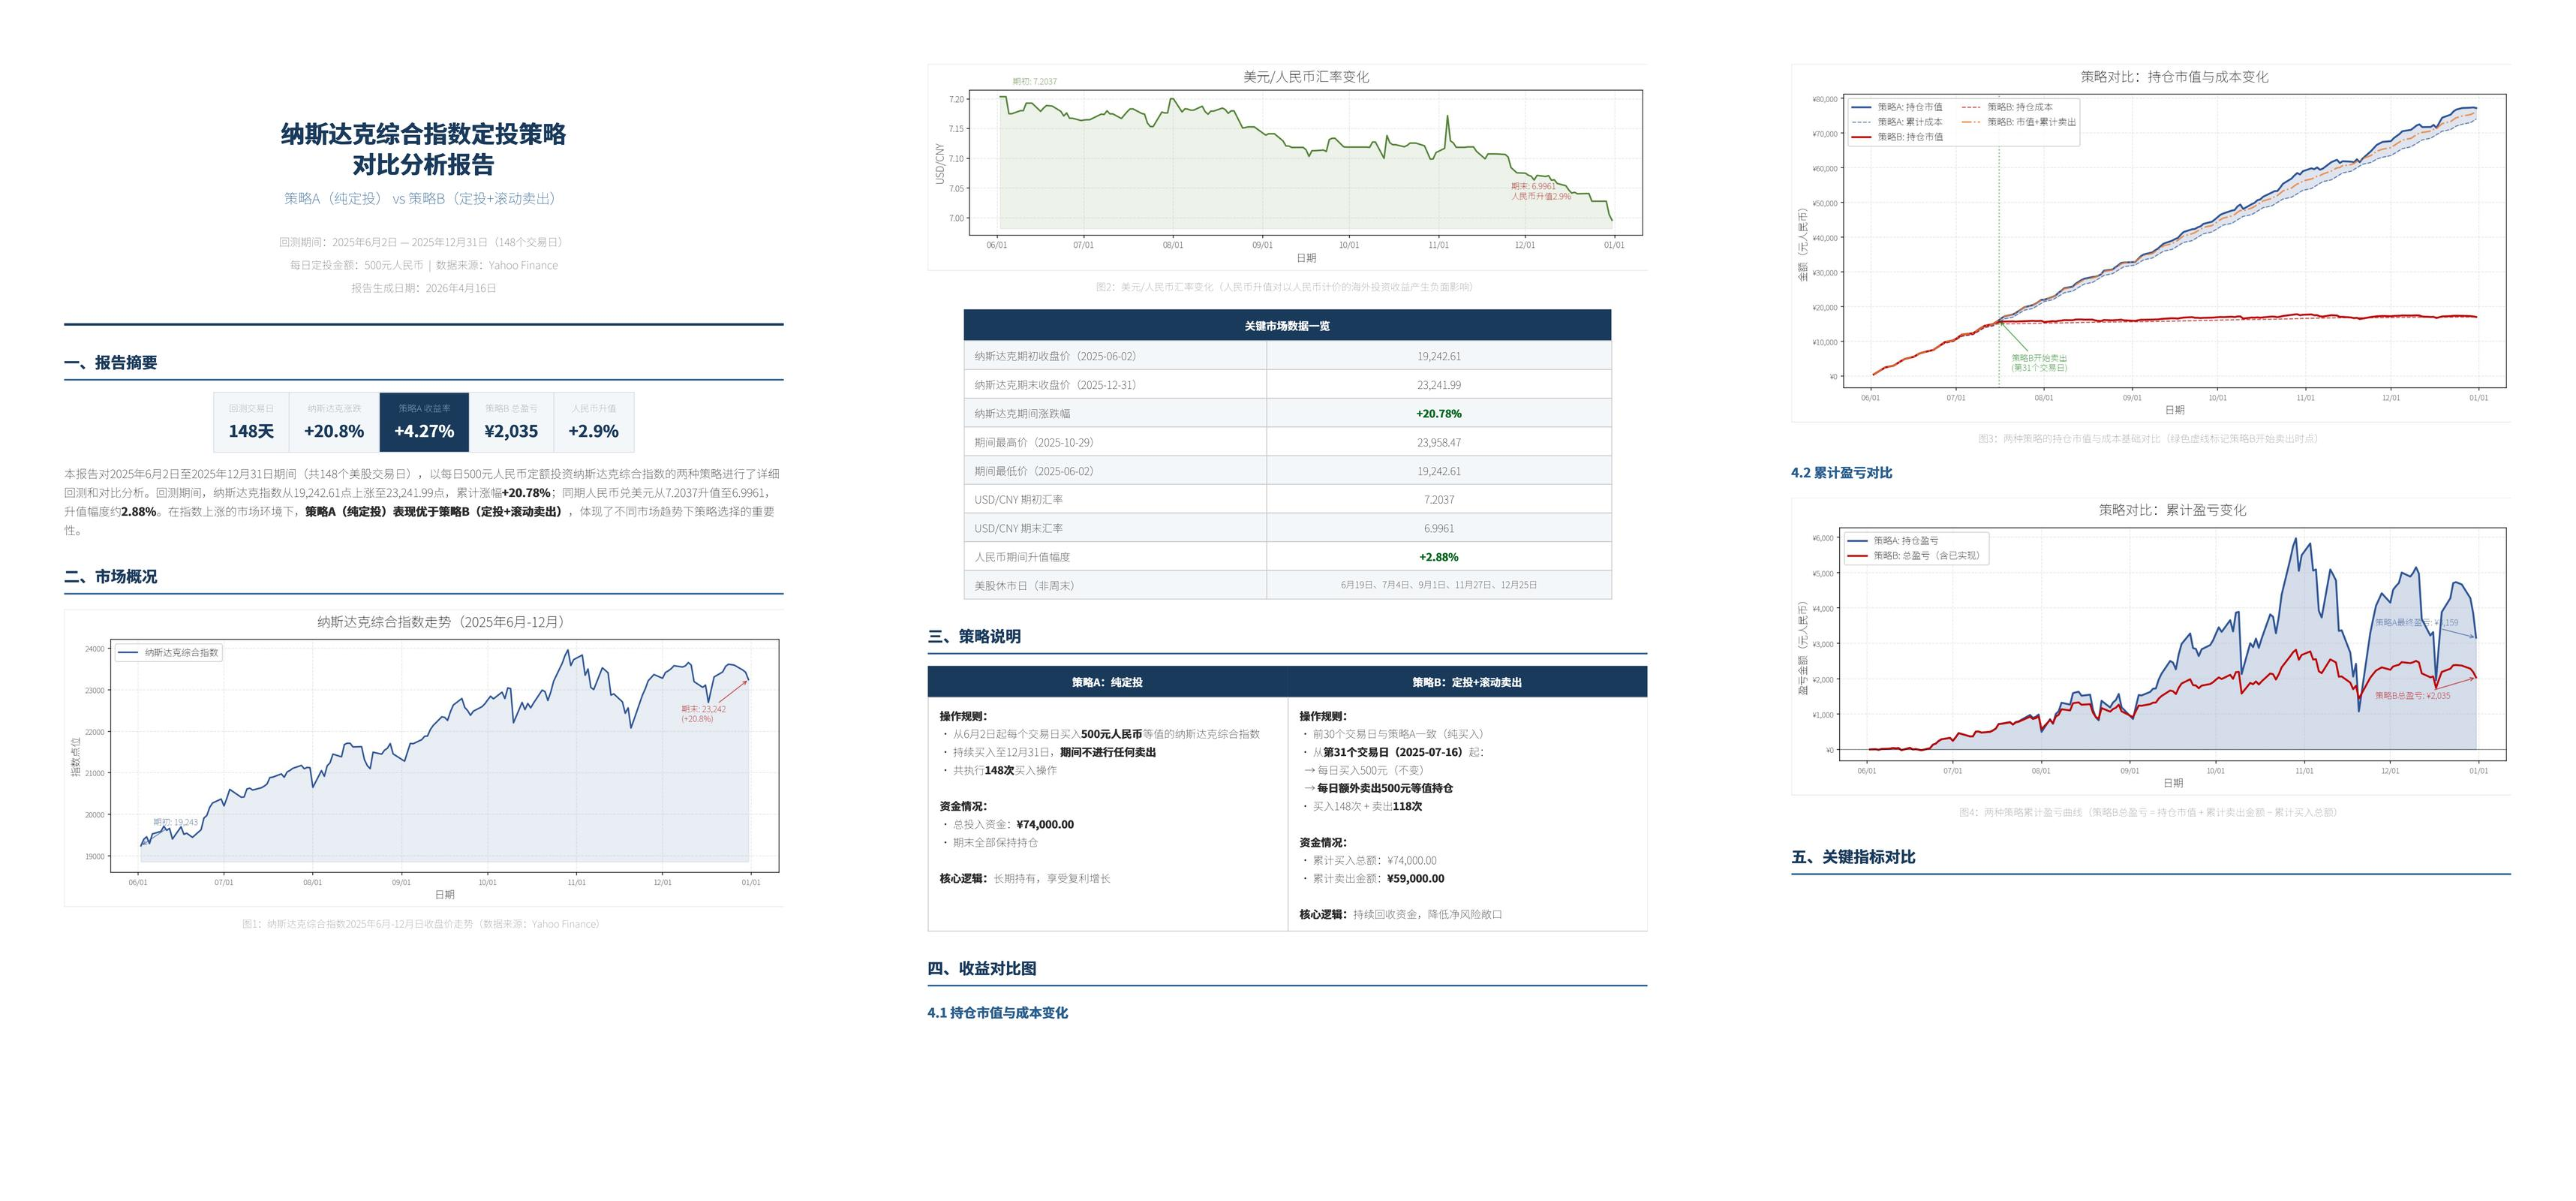
\includegraphics[keepaspectratio,alt={image}]{images_hi/p56-000.jpg}}

图 14 \textbar{} 需要比较纳斯达克两种定投策略的任务输出示例。

\pandocbounded{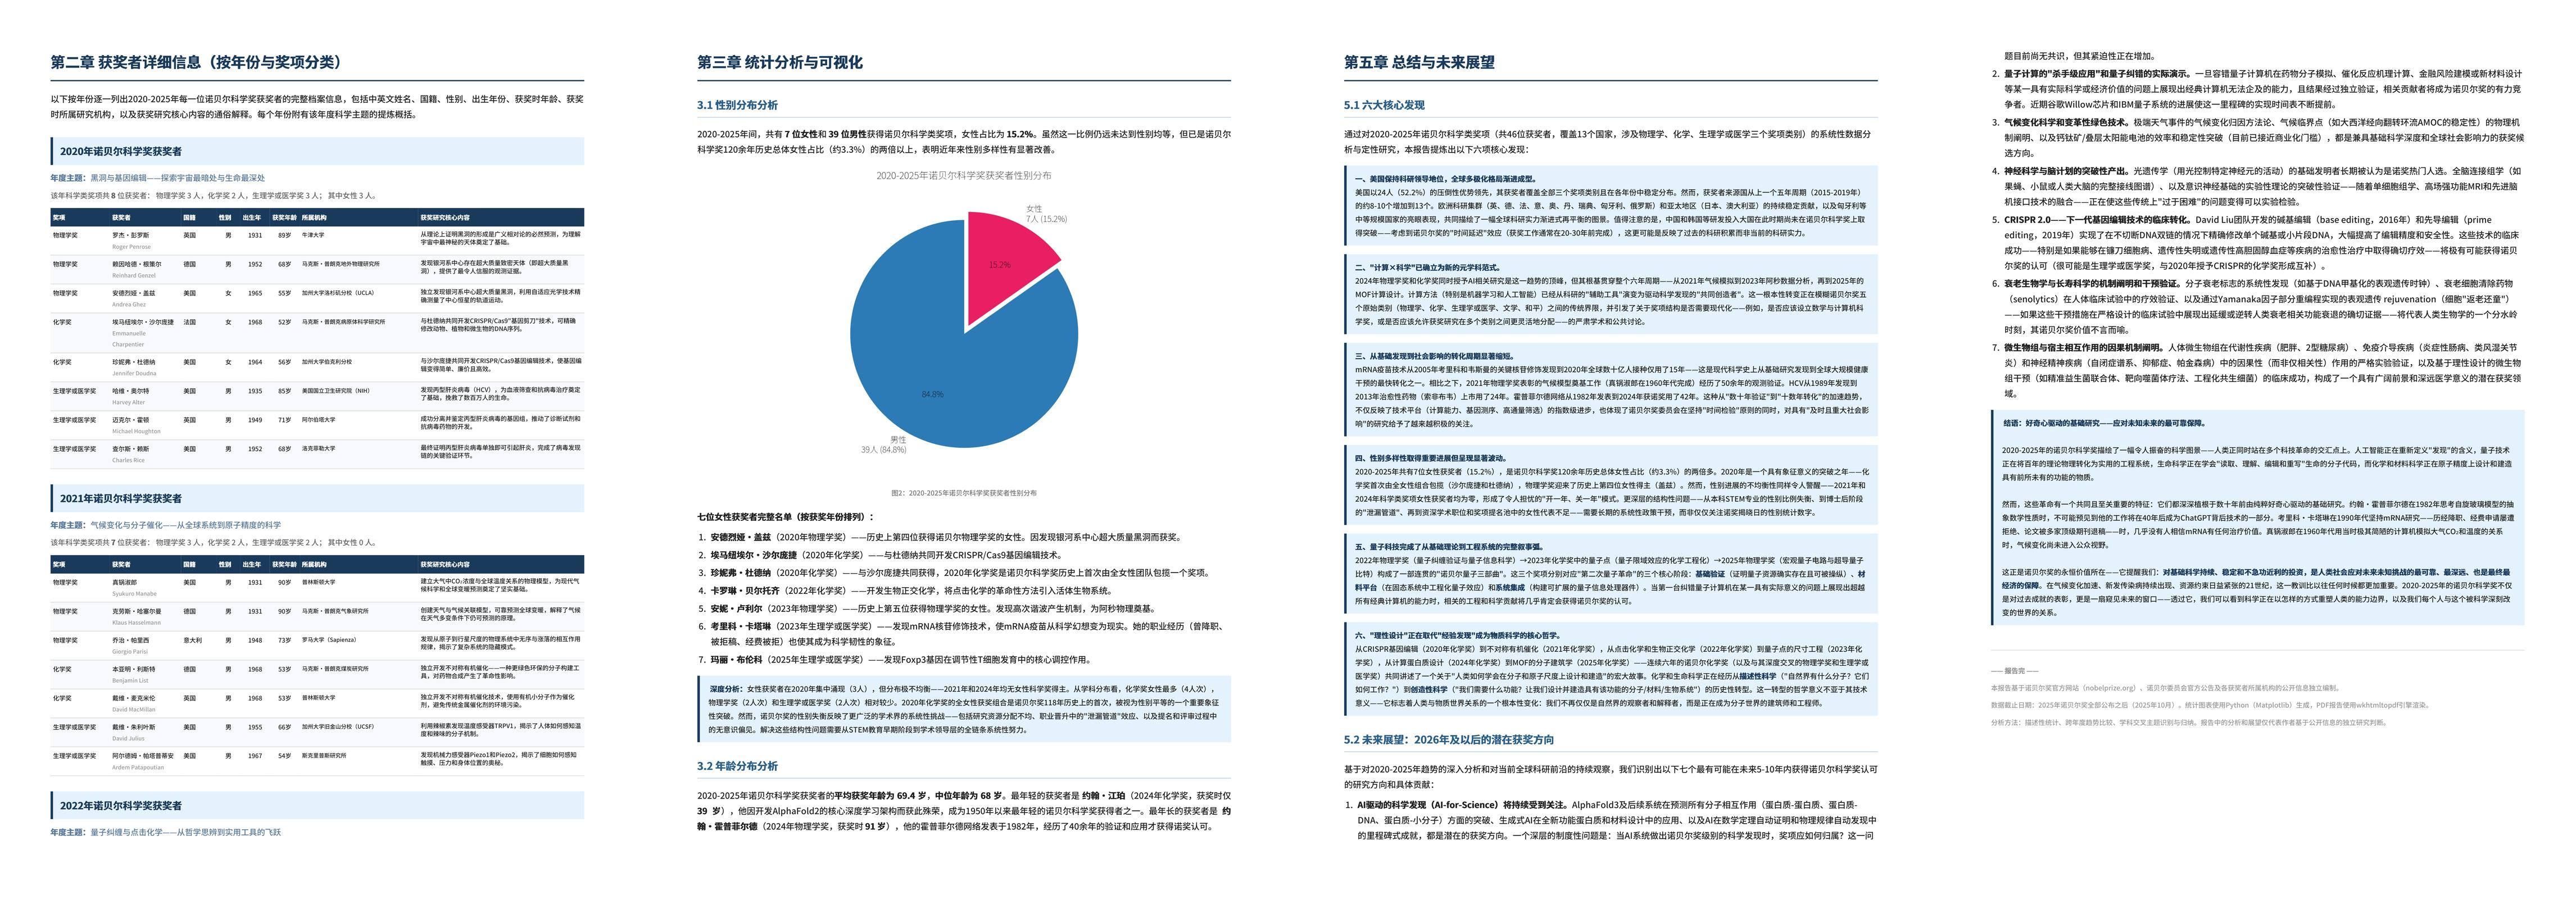
\includegraphics[keepaspectratio,alt={image}]{images_hi/p56-001.jpg}}

图 15 \textbar{} 需要调研 2020-2025 年诺贝尔科学奖并生成分析型 PDF 报告的任务输出示例。

表 12 \textbar{} DeepSeek-V4-Pro 与 Gemini-3.1-Pro 在中文功能性写作上的对比分析。

{\def\LTcaptype{none} % do not increment counter
\begin{longtable}[]{@{}lllllllll@{}}
\toprule\noalign{}
\endhead
\bottomrule\noalign{}
\endlastfoot
\multirow{2}{*}{Category} & \multirow{2}{*}{Subcategory} &
\multirow{2}{*}{\#} & \multicolumn{6}{l@{}}{%
Internal Evaluation (内部综合评估)} \\
& & & DS win & Gem win & Tie & DS\% & Gem\% & Tie\% \\
\multirow{10}{*}{Business Writing (办公文本)} & Report (报告) & 527 &
350 & 162 & 15 & 66.41 & 30.74 & 2.85 \\
& Proposal (方案策划) & 291 & 181 & 103 & 7 & 62.20 & 35.40 & 2.41 \\
& Education (教育培训) & 159 & 100 & 56 & 3 & 62.89 & 35.22 & 1.89 \\
& Email \& Letter (邮件书信) & 146 & 107 & 37 & 2 & 73.29 & 25.34 &
1.37 \\
& Notice (通知公告) & 72 & 43 & 24 & 5 & 59.72 & 33.33 & 6.94 \\
& Professional (专业文本) & 63 & 34 & 27 & 2 & 53.97 & 42.86 & 3.17 \\
& Recruitment (招聘求职) & 42 & 27 & 15 & 0 & 64.29 & 35.71 & 0.00 \\
& Technical (技术文本) & 29 & 22 & 7 & 0 & 75.86 & 24.14 & 0.00 \\
& Review (介绍评价) & 20 & 15 & 5 & 0 & 75.00 & 25.00 & 0.00 \\
& Subtotal (小计) & 1349 & 879 & 436 & 34 & 65.16 & 32.32 & 2.52 \\
\multirow{9}{*}{Media Writing (媒体文本)} & Social Media (社交媒体文案)
& 267 & 156 & 101 & 10 & 58.43 & 37.83 & 3.75 \\
& Ad Copy (广告商品文案) & 214 & 109 & 98 & 7 & 50.93 & 45.79 & 3.27 \\
& Long-form Content (内容平台长文) & 99 & 71 & 25 & 3 & 71.72 & 25.25 &
3.03 \\
& News Report (新闻报道) & 51 & 27 & 22 & 2 & 52.94 & 43.14 & 3.92 \\
& Advertorial (营销软文) & 17 & 12 & 4 & 1 & 70.59 & 23.53 & 5.88 \\
& Headline (标题) & 11 & 7 & 4 & 0 & 63.64 & 36.36 & 0.00 \\
& Narration Script (口播文案) & 4 & 2 & 1 & 1 & 50.00 & 25.00 & 25.00 \\
& Comment (评论) & 3 & 2 & 1 & 0 & 66.67 & 33.33 & 0.00 \\
& Subtotal (小计) & 666 & 386 & 256 & 24 & 57.96 & 38.44 & 3.60 \\
\multirow{6}{*}{Everyday Writing (生活文本)} & Congratulatory (祝贺文本)
& 101 & 54 & 41 & 6 & 53.47 & 40.59 & 5.94 \\
& Communication (沟通回复) & 100 & 71 & 26 & 3 & 71.00 & 26.00 & 3.00 \\
& Reflection (心得感想) & 90 & 68 & 17 & 5 & 75.56 & 18.89 & 5.56 \\
& Review (介绍评价) & 55 & 44 & 9 & 2 & 80.00 & 16.36 & 3.64 \\
& Comment (评论) & 44 & 34 & 8 & 2 & 77.27 & 18.18 & 4.55 \\
& Subtotal (小计) & 390 & 271 & 101 & 18 & 69.49 & 25.90 & 4.62 \\
\multirow{6}{*}{Oral Writing (口头文本)} & Speech (发言稿) & 226 & 135 &
85 & 6 & 59.73 & 37.61 & 2.65 \\
& Narration Script (口播文案) & 51 & 25 & 23 & 3 & 49.02 & 45.10 &
5.88 \\
& Sales Script (话术) & 31 & 22 & 6 & 3 & 70.97 & 19.35 & 9.68 \\
& Dialogue (对话文本) & 10 & 4 & 6 & 0 & 40.00 & 60.00 & 0.00 \\
& Congratulatory (祝贺文本) & 1 & 1 & 0 & 0 & 100.00 & 0.00 & 0.00 \\
& Subtotal (小计) & 319 & 187 & 120 & 12 & 58.62 & 37.62 & 3.76 \\
\multirow{6}{*}{Official Document (公文文本)} & Administrative Doc
(事务文书) & 117 & 60 & 53 & 4 & 51.28 & 45.30 & 3.42 \\
& Personal Doc (个人文书) & 73 & 45 & 27 & 1 & 61.64 & 36.99 & 1.37 \\
& Government Doc (行政公文) & 34 & 19 & 14 & 1 & 55.88 & 41.18 & 2.94 \\
& Speech (发言稿) & 3 & 1 & 2 & 0 & 33.33 & 66.67 & 0.00 \\
& Essay Writing (申论写作) & 3 & 1 & 1 & 1 & 33.33 & 33.33 & 33.33 \\
& Subtotal (小计) & 230 & 126 & 97 & 7 & 54.78 & 42.17 & 3.04 \\
\multirow{5}{*}{Academic Writing (学术文本)} & Research Paper (学术论文)
& 104 & 67 & 32 & 5 & 64.42 & 30.77 & 4.81 \\
& Coursework (课程作业) & 90 & 53 & 35 & 2 & 58.89 & 38.89 & 2.22 \\
& Academic Support (学术辅助) & 15 & 11 & 3 & 1 & 73.33 & 20.00 &
6.67 \\
& Science Outreach (专业科普) & 7 & 6 & 1 & 0 & 85.71 & 14.29 & 0.00 \\
& Subtotal (小计) & 216 & 137 & 71 & 8 & 63.43 & 32.87 & 3.70 \\
Total (总计) & & 3170 & 1986 & 1081 & 103 & 62.65 & 34.10 & 3.25 \\
\end{longtable}
}

表 13 \textbar{} DeepSeek-V4-Pro 与 Gemini-3.1-Pro 在中文创意写作上的对比分析。

{\def\LTcaptype{none} % do not increment counter
\begin{longtable}[]{@{}llllllllllllll@{}}
\toprule\noalign{}
\endhead
\bottomrule\noalign{}
\endlastfoot
\multirow{2}{*}{Subcategory (文体)} & \multirow{2}{*}{\#} &
\multicolumn{6}{l}{%
Instruction Following(指令遵循)} & \multicolumn{6}{l@{}}{%
Writing Quality (写作质量)} \\
& & DS & Gem & Tie & DS\% & Gem\% & Tie\% & DS & Gem & Tie & DS\% &
Gem\% & Tie\% \\
Fiction (小说故事) & 836 & 504 & 323 & 5 & 60.58 & 38.82 & 0.60 & 672 &
157 & 3 & 80.77 & 18.87 & 0.36 \\
General Fiction (泛小说故事) & 662 & 368 & 290 & 3 & 55.67 & 43.87 &
0.45 & 467 & 194 & 0 & 70.65 & 29.35 & 0.00 \\
Fan Fiction (同人文) & 410 & 253 & 150 & 3 & 62.32 & 36.95 & 0.74 & 338
& 67 & 1 & 83.25 & 16.50 & 0.25 \\
General Fan Fic. (泛同人文) & 202 & 111 & 90 & 1 & 54.95 & 44.55 & 0.50
& 161 & 40 & 1 & 79.70 & 19.80 & 0.50 \\
Narrative (记叙文) & 171 & 115 & 54 & 2 & 67.25 & 31.58 & 1.17 & 141 &
30 & 0 & 82.46 & 17.54 & 0.00 \\
General Prose (泛散文) & 124 & 83 & 40 & 1 & 66.94 & 32.26 & 0.81 & 88 &
36 & 0 & 70.97 & 29.03 & 0.00 \\
Prose (散文) & 112 & 74 & 38 & 0 & 66.07 & 33.93 & 0.00 & 92 & 20 & 0 &
82.14 & 17.86 & 0.00 \\
Writing Style (文笔) & 112 & 81 & 31 & 0 & 72.32 & 27.68 & 0.00 & 86 &
26 & 0 & 76.79 & 23.21 & 0.00 \\
Classical Poetry (古诗文) & 48 & 24 & 24 & 0 & 50.00 & 50.00 & 0.00 & 39
& 9 & 0 & 81.25 & 18.75 & 0.00 \\
Modern Poetry (现代诗) & 43 & 23 & 20 & 0 & 53.49 & 46.51 & 0.00 & 32 &
11 & 0 & 74.42 & 25.58 & 0.00 \\
Lyrics (歌词) & 30 & 8 & 22 & 0 & 26.67 & 73.33 & 0.00 & 16 & 14 & 0 &
53.33 & 46.67 & 0.00 \\
Literary Appreciation (赏析) & 27 & 20 & 7 & 0 & 74.07 & 25.93 & 0.00 &
18 & 9 & 0 & 66.67 & 33.33 & 0.00 \\
General Argument. (泛议论文) & 24 & 15 & 9 & 0 & 62.50 & 37.50 & 0.00 &
17 & 7 & 0 & 70.83 & 29.17 & 0.00 \\
General Narrative (泛记叙文) & 23 & 11 & 12 & 0 & 47.83 & 52.17 & 0.00 &
15 & 8 & 0 & 65.22 & 34.78 & 0.00 \\
General Classical (泛古文诗歌) & 9 & 5 & 4 & 0 & 55.56 & 44.44 & 0.00 &
5 & 4 & 0 & 55.56 & 44.44 & 0.00 \\
Creative Writing (创意写作) & 6 & 2 & 4 & 0 & 33.33 & 66.67 & 0.00 & 4 &
2 & 0 & 66.67 & 33.33 & 0.00 \\
Argumentative (议论文) & 5 & 5 & 0 & 0 & 100.00 & 0.00 & 0.00 & 5 & 0 &
0 & 100.00 & 0.00 & 0.00 \\
General Mod. Poetry (泛现代诗) & 2 & 1 & 1 & 0 & 50.00 & 50.00 & 0.00 &
2 & 0 & 0 & 100.00 & 0.00 & 0.00 \\
Total (总计) & 2837 & 1703 & 1119 & 15 & 60.03 & 39.44 & 0.53 & 2198 &
634 & 5 & 77.48 & 22.35 & 0.18 \\
\end{longtable}
}

表 14 \textbar{} DeepSeek-V4-Pro 与 Claude-Opus-4.5 在复杂指令遵循与多轮写作上的对比。

{\def\LTcaptype{none} % do not increment counter
\begin{longtable}[]{@{}llllllll@{}}
\toprule\noalign{}
\endhead
\bottomrule\noalign{}
\endlastfoot
\multirow{2}{*}{Category} & \multirow{2}{*}{\#} &
\multicolumn{6}{l@{}}{%
Internal Evaluation (内部综合评估)} \\
& & DS & Opus & Tie & DS\% & Opus\% & Tie\% \\
Complex Inst. Following (复杂指令跟随) & 49 & 23 & 26 & 0 & 46.9\% &
53.1\% & 0.0\% \\
Multi-Turn Writing (多轮写作) & 147 & 67 & 76 & 4 & 45.6\% & 51.7\% &
2.7\% \\
Total (总计) & 196 & 90 & 102 & 4 & 45.9\% & 52.0\% & 2.0\% \\
\end{longtable}
}


\end{document}
